%% Adaptado a partir de :
%%    abtex2-modelo-trabalho-academico.tex, v-1.9.2 laurocesar
%% para ser um modelo para os trabalhos no IFSP-SPO

\documentclass[
    % -- opções da classe memoir --
    12pt,               % tamanho da fonte
    openright,          % capítulos começam em pág ímpar (insere página vazia caso preciso)
    %twoside,            % para impressão em verso e anverso. Oposto a oneside
    oneside,
    a4paper,            % tamanho do papel. 
    % -- opções da classe abntex2 --schwinn
    % Opções que não devem ser utilizadas na versão final do documento
    %draft,              % para compilar mais rápido, remover na versão final
    paginasA3,  % indica que vai utilizar paginas em A3 
    MODELO,             % indica que é um documento modelo então precisa dos geradores de texto
    TODO,               % indica que deve apresentar lista de pendencias 
    % -- opções do pacote babel --
    english,            % idioma adicional para hifenização
    brazil              % o último idioma é o principal do documento
    ]{ifsp-spo-inf-ctds} % ajustar de acordo com o modelo desejado para o curso


% ---
% Informações de dados para CAPA e FOLHA DE ROSTO
% ---
\titulo{Análise Exploratória de Dados (EDA) \\ Estudo de Caso}

% Trabalho individual
%\autor{AUTOR DO TRABALHO}

% Trabalho em Equipe
% ver também https://github.com/abntex/abntex2/wiki/FAQ#como-adicionar-mais-de-um-autor-ao-meu-projeto
\renewcommand{\imprimirautor}{
\begin{tabular}{lr}
Leonardo Naoki Narita & SP3022498 
\end{tabular}
}


\disciplina{PFUEL - Programação Funcional}

\preambulo{Trabalho desenvolvido no curso de Tecnologia
em Análise e Desenvolvimento de Sistemas
do Instituto Federal de Educação, Ciência e
Tecnologia de São Paulo como requisito parcial
para a conclusão da disciplina de Programação Funcional.}

\data{27 de Janeiro de 2022}

% Definir o que for necessário e comentar o que não for necessário
% Utilizar o Nome Completo, abntex tem orientador e coorientador
% então vão ser utilizados na definição de professor
\renewcommand{\orientadorname}{Professor:}
\orientador{Guilherme Werneck de Oliveira}


% ---


% informações do PDF
\makeatletter
\hypersetup{
        %pagebackref=true,
        pdftitle={\@title}, 
        pdfauthor={\@author},
        pdfsubject={\imprimirpreambulo},
        pdfcreator={LaTeX with abnTeX2 using IFSP model},
        pdfkeywords={abnt}{latex}{abntex}{abntex2}{IFSP}{\ifspprefixo}{trabalho acadêmico}, 
        colorlinks=true,            % false: boxed links; true: colored links
        linkcolor=blue,             % color of internal links
        citecolor=blue,             % color of links to bibliography
        filecolor=magenta,              % color of file links
        urlcolor=blue,
        bookmarksdepth=4
}
\makeatother
% --- 

\graphicspath{ {./images} }
\usepackage{float}

% carregando aqui referencias quando utilizando BIBLATEX
\IfPackageLoaded{biblatex}{%
\addbibresource{referencias.bib}
\addbibresource{exemplos/abntex2-doc-abnt-6023.bib}
}{}

% ----
% Início do documento
% ----
\begin{document}


% Retira espaço extra obsoleto entre as frases.
\frenchspacing 

% -- lista de pendencias gerada pelo todonotes
% -- altere opções do usepackage para remover na versão final....
%\listoftodos
%\todo[inline]{remover lista de todo da versão final...}

\newpage

% ----------------------------------------------------------
% ELEMENTOS PRÉ-TEXTUAIS
% ----------------------------------------------------------
\pretextual

% ---
% Capa
% ---
\imprimircapa
\newcounter{todocounter}
\newcommand{\todonum}[2][]
{\stepcounter{todocounter}\todo[#1]{\thetodocounter: #2}}


% ---

% ---
% Folha de rosto
% (o * indica que haverá a ficha bibliográfica)
% ---
\imprimirfolhaderosto

%\todo[inline]{colocar a data de entrega}

%\imprimirfolhaderosto*
% ---

% Quando registrado na biblioteca
%
% ---
% Inserir a ficha bibliografica
% ---

% Isto é um exemplo de Ficha Catalográfica, ou ``Dados internacionais de
% catalogação-na-publicação''. Você pode utilizar este modelo como referência. 
% Porém, provavelmente a biblioteca da sua universidade lhe fornecerá um PDF
% com a ficha catalográfica definitiva após a defesa do trabalho. Quando estiver
% com o documento, salve-o como PDF no diretório do seu projeto e substitua todo
% o conteúdo de implementação deste arquivo pelo comando abaixo:
%
% \begin{fichacatalografica}
%     \includepdf{fig_ficha_catalografica.pdf}
% \end{fichacatalografica}
\begin{fichacatalografica}
    \vspace*{\fill}                 % Posição vertical
    \hrule                          % Linha horizontal
    \begin{center}                  % Minipage Centralizado
    \begin{minipage}[c]{12.5cm}     % Largura
    
    \imprimirautor
    
    \hspace{0.5cm} \imprimirtitulo  / \imprimirautor. --
    \imprimirlocal, \imprimirdata-
    
    \hspace{0.5cm} \pageref{LastPage} p. : il. (algumas color.) ; 30 cm.\\
    
    \hspace{0.5cm} \imprimirorientadorRotulo~\imprimirorientador\\
    
    \hspace{0.5cm}
    \parbox[t]{\textwidth}{\imprimirtipotrabalho~--~\imprimirinstituicao,
    \imprimirdata.}\\
    
    \hspace{0.5cm}
        1. Palavra-chave1.
        2. Palavra-chave2.
        I. Orientador.
        II. Universidade xxx.
        III. Faculdade de xxx.
        IV. Título\\            
    
    \hspace{8.75cm} CDU 02:141:005.7\\
    
    \end{minipage}
    \end{center}
    \hrule
\end{fichacatalografica}
% ---



%Caso necessário
%% ---
% Inserir errata
% ---
\begin{errata}
Elemento opcional da \citeonline[4.2.1.2]{NBR14724:2011}. Exemplo:

\vspace{\onelineskip}


FERRIGNO, C. R. A. \textbf{Tratamento de neoplasias ósseas apendiculares com
reimplantação de enxerto ósseo autólogo autoclavado associado ao plasma
rico em plaquetas}: estudo crítico na cirurgia de preservação de membro em
cães. 2011. 128 f. Tese (Livre-Docência) - Faculdade de Medicina Veterinária e
Zootecnia, Universidade de São Paulo, São Paulo, 2011.

\begin{table}[htb]
\center
\footnotesize
\begin{tabular}{|p{1.4cm}|p{1cm}|p{3cm}|p{3cm}|}
  \hline
   \textbf{Folha} & \textbf{Linha}  & \textbf{Onde se lê}  & \textbf{Leia-se}  \\
    \hline
    1 & 10 & auto-conclavo & autoconclavo\\
   \hline
\end{tabular}
\end{table}

\end{errata}
% ---

%Obrigatório para trabalhos com bancas oficiais
%% ---
% Inserir folha de aprovação
% ---

% Isto é um exemplo de Folha de aprovação, elemento obrigatório da NBR
% 14724/2011 (seção 4.2.1.3). Você pode utilizar este modelo até a aprovação
% do trabalho. Após isso, substitua todo o conteúdo deste arquivo por uma
% imagem da página assinada pela banca com o comando abaixo:
%
% \includepdf{folhadeaprovacao_final.pdf}
%
\begin{folhadeaprovacao}

  \begin{center}
    {\ABNTEXchapterfont\large\imprimirautor}

    \vspace*{\fill}\vspace*{\fill}
    \begin{center}
      \ABNTEXchapterfont\bfseries\Large\imprimirtitulo
    \end{center}
    \vspace*{\fill}
    
    \hspace{.45\textwidth}
    \begin{minipage}{.5\textwidth}
        \imprimirpreambulo
    \end{minipage}%
    \vspace*{\fill}
   \end{center}
        
   Trabalho aprovado. \imprimirlocal, 24 de novembro de 2012:

   \assinatura{\textbf{\imprimirorientador} \\ Orientador} 
   \assinatura{\textbf{Professor} \\ Convidado 1}
   \assinatura{\textbf{Professor} \\ Convidado 2}
   %\assinatura{\textbf{Professor} \\ Convidado 3}
   %\assinatura{\textbf{Professor} \\ Convidado 4}
      
   \begin{center}
    \vspace*{0.5cm}
    {\large\imprimirlocal}
    \par
    {\large\imprimirdata}
    \vspace*{1cm}
  \end{center}
  
\end{folhadeaprovacao}
% ---



% ---
% inserir lista de ilustrações
% ---
%\pdfbookmark[0]{\listfigurename}{lof}
%\listoffigures*
%\cleardoublepage
% ---

% ---
% inserir lista de tabelas
% ---
%\pdfbookmark[0]{\listtablename}{lot}
%\listoftables*
%\cleardoublepage
% ---

% ---
% inserir lista de quadros
% ---
%\pdfbookmark[0]{\listofquadrosname}{loq}
%\listofquadros*
%\cleardoublepage
% ---


% ---
% inserir o sumario
% ---
\pdfbookmark[0]{\contentsname}{toc}
\tableofcontents*
\cleardoublepage
% ---


% ----------------------------------------------------------
% ELEMENTOS TEXTUAIS
% ----------------------------------------------------------
\textual

\chapter{Introdução}	

Nesse capítulo, são abordados conceitos fundamentais que embasam o desenvolvimento do projeto.

\section{Definição de EDA}

A Análise Exploratória de Dados (do inglês, "Exploratory Data Analysis", conhecida também pela sigla "EDA") é a aplicação de um conjunto de técnicas que visam analisar uma população ou amostra de dados (conjunto de dados dentro de um mesmo contexto).

A EDA visa identificar conclusões significativas dentro dessa massa de dados, podendo ser padrões ou outliers (inconsistências de dados).

\section{Ciclo de Vida da EDA}

Dado que há uma massa de dados importada e devidamente tratada (tendo-os consistentes), o ciclo de vida da EDA baseia-se em três passos:

\subsection{Gerar Questionamentos}

O primeiro passo é gerar questionamentos sobre os dados que estão dispostos, criando variáveis e agregações.

Para gerar questionamentos, uma questão é fundamental a ser indagada: "Que tipo de variação ocorre com as variáveis?".

\subsection{Modelas Dados}

O segundo passo é organizar os dados de modo que seja visualmente fácil de analisar para que, assim possa encontrar conclusões.

\subsection{Buscar Conclusões}

O terceiro e último passo é analisar as conclusões obtidas, podendo chegar a novos questionamentos.






\chapter{Apresentação do Conjunto de Dados}	

Nesse capítulo, é definida a massa de dados a ser importado no projeto, bem como suas variáveis e detalhes.

\section{Escolha dos Dados}

O conjunto de dados escolhidos para o projeto é o "Brazilian Cites", onde há 5573 cidades brasileiras, disponível em: https://www.kaggle.com/crisparada/brazilian-cities.

\section{Dicionário de Dados}

Nessa seção, é definido os principais atributos que serão trabalhados e analisados pela EDA. 

Os principais atributos das cidades do Brasil, dispostas na planilha, são:

\begin{quadro}[H]
\centering
\ABNTEXfontereduzida
\caption[Definição dos Principais Atributos]{Definição dos Principais Atributos}
\label{dicionario-dados-globalcomment}
\begin{tabular}{|p{5.0cm}|p{5.0cm}|p{5.0cm}|}

  \hline
  \multicolumn{3}{|c|}{Cidades do Brasil} \\
  
  \hline
  \thead{Atributo} & \thead{Descrição}  & \thead{Valores} \\
    
  \hline 
  CITY & Nome da cidade &  \\
  
  \hline 
  STATE & Nome do estado &  \\

  \hline 
  CAPITAL & Indica se a cidade é a capital do estado & 1 (SIM) ou 0 (NÃO) \\
  
  \hline 
  IBGE\_RES\_POP & População residente na cidade &  \\
  
  \hline 
  IBGE\_RES\_POP\_BRAS & População brasileira residente na cidade &  \\
  
  \hline 
  IBGE\_RES\_POP\_ESTR & População estrangeira residente na cidade &  \\
  
  \hline 
  IDHM & Índice de Desenvolvimento Humano (IDH) &  \\
  
  \hline 
  IDHM\_Renda & Índice de renda pelo IDH &  \\
  
  \hline 
  IDHM\_Longevidade & Índice de longevidade pelo IDH &  \\
  
  \hline 
  IDHM\_Educacao & Índice de educação pelo IDH &  \\
  
  \hline
\end{tabular}
\legend{Fonte: \href{https://www.kaggle.com/crisparada/brazilian-cities?select=Data_Dictionary.csv}{Kaggle}}
\end{quadro}


\chapter{Desenvolvimento da EDA}

Nesse capítulo, é aplicado os três passos do ciclo de uma EDA em um contexto prático aplicando o conjunto de dados "Brazilian Cities".

\section{Caso 1: Análise do IDH}

O IDH (Índice de Desenvolvimento Humano) é um índice que avalia a qualidade de vida em um determinado local, sendo mensurado a partir de 3 fatores: Longevidade, Educação e Renda. No Brasil, o órgão responsável por avaliar o IDH é o IBGE (Instituto Brasileiro de Geografia e Estatística).

Sendo um parâmetro importante, o IDH é capaz de influenciar tomadas de decisões, tais como quais setores aplicar investimento público pelos políticos, se é vantajoso mudar-se para morar nesse local, e se é viável a iniciativa privada investir nesse local para atuar.

Vide na figura \autoref{fig:distribuicao-idh-nas-cidades} a distribuição do IDH nas cidades do Brasil.

\begin{figure}[H]
  \centering
  \caption{\label{fig:distribuicao-idh-nas-cidades}Distribuição do IDH nas cidades brasileiras}
  \label{fig:der}
  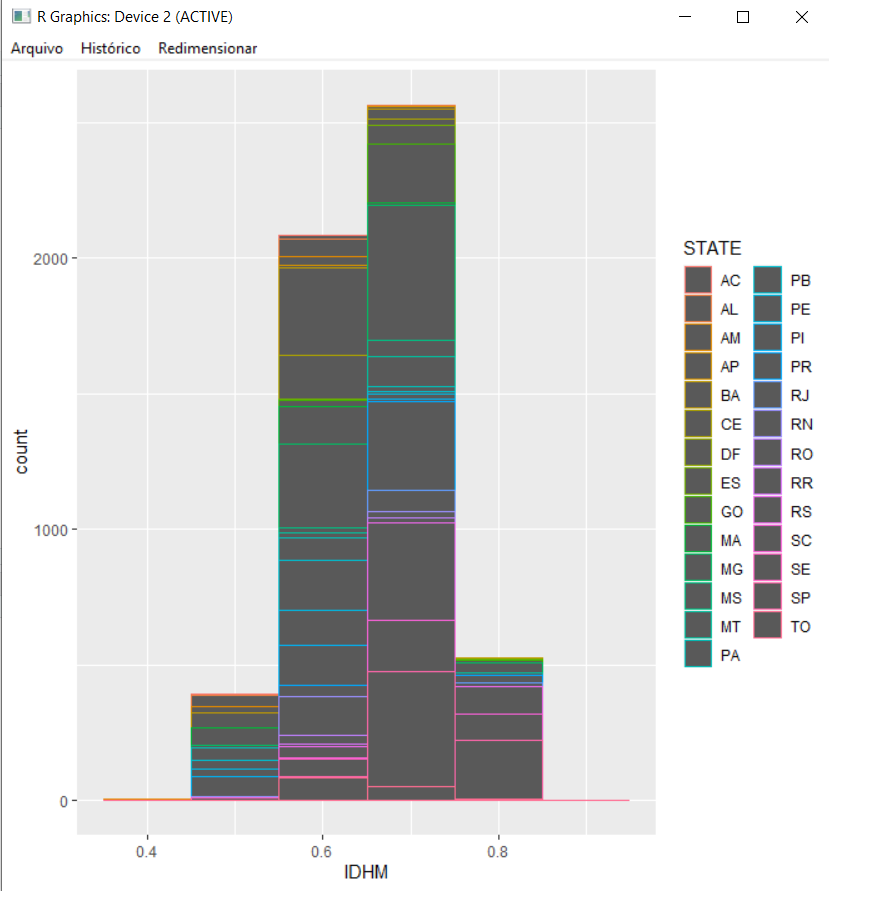
\includegraphics[scale=0.6]{chapter-03-case-01-img-01}
  \legend{Fonte: O autor}
\end{figure}

Visualizando esse gráfico, é perceber que não há cidades brasileiras com IDH menor do que 0.4, nem com IDH maior do que 0.8.

Com isso, surgem-se duas questões: 

\begin{enumerate}
	\item "Por que não existe IDH maior que 1?";
	\item "Q2?".
\end{enumerate}	

...

\section{Caso 2: Análise de Estrangeiros}

No mesmo contexto do caso 1, outra questão deve ser feita: "Um estrangeiro, de modo geral, reside em cidades com maiores índices de IDH ou cidades mais populosas?".

Na figura \autoref{fig:idh-x-estrangeiro}, revela a distribuição dos estrangeiros residentes por IDH.

\begin{figure}[H]
  \centering
  \caption{\label{fig:idh-x-estrangeiro}Distribuição de estrangeiros por IDH}
  \label{fig:der}
  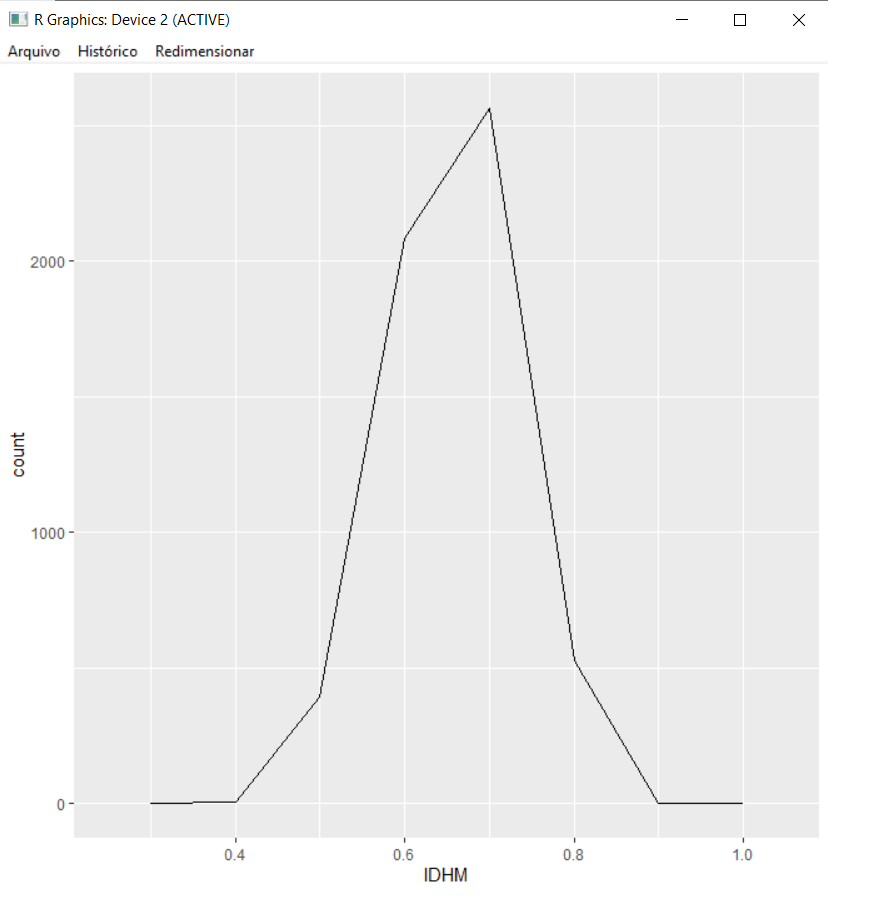
\includegraphics[scale=0.6]{chapter-03-case-02-img-01}
  \legend{Fonte: O autor}
\end{figure}

Já na figura, é mostrado a distribuição da população estrangeira sobre a população total de uma cidade.

...






\chapter{Conclusão}



% ----------------------------------------------------------
% Finaliza a parte no bookmark do PDF
% para que se inicie o bookmark na raiz
% e adiciona espaço de parte no Sumário
% ----------------------------------------------------------
\phantompart

% ----------------------------------------------------------
% ELEMENTOS PÓS-TEXTUAIS
% ----------------------------------------------------------
\postextual
% ----------------------------------------------------------

% ----------------------------------------------------------
% Referências bibliográficas
% ----------------------------------------------------------
% quando não esta utilizando biblatex tem que carregar as referencias aqui

%
%\IfPackageLoaded{biblatex}{}{%
%\bibliography{referencias/referencias}
%}

%% ----------------------------------------------------------
% Anexos
% Documentos gerados por outros autores
% ----------------------------------------------------------

% ---
% Inicia os anexos
% ---
\begin{anexosenv}
\anexos
% Imprime uma página indicando o início dos anexos
\partanexos

% ---
\chapter{Manual todonotes(parcial)}
\label{manual-todonotes}
% ---
\index{pdf}
% se pages = "-"  fica com arquivo completo
\includepdf[pages=1-3,scale=0.8,frame=true,pagecommand={}]{anexos/todonotes.pdf}

% ---
% Para incluir sem gerar a quebra de página inicial no anexo
\includepdf[pages=1,scale=0.7,frame=true,pagecommand=\chapter{Manual pdfpages(parcial)}\label{manual-pdfpages}]{anexos/pdfpages.pdf}
\includepdf[pages=2-3,scale=0.8,frame=true,pagecommand={}]{anexos/pdfpages.pdf}

% ---
\chapter{Manual acronym(parcial)}
\index{pdf}
% somente algumas páginas para exemplo sem borda
\includepdf[pages=1-3,frame=false,pagecommand={}]{anexos/acronym.pdf}



\includepdf[frame=true,scale=0.7,pagecommand=\chapter{Referência Rápida pifont}\label{pifont-quickref}]{anexos/pifont.pdf}


\end{anexosenv}


%---------------------------------------------------------------------

\end{document}